\chapter{色と見た目を変える}
\label{chap:color-and-style}

この章では、図形の色、枠線、塗りつぶし、線の太さを変える方法を学びます。第2章では図形の形と位置を中心に扱いました。ここでは、同じ図形でも色や線の指定によって印象が大きく変わることを確認します。

\section{この章の概要}

p5.jsでは、図形を描く前に色や線の設定を行います。設定した色や線の太さは、次に別の設定をするまで残ります。この「設定が残る」という考え方を理解すると、複数の図形を意図した見た目で描けるようになります。

この章で扱う主な内容は次の通りです。

\begin{itemize}
    \item RGBによる色の指定
    \item 灰色系の簡単な指定
    \item \texttt{fill}による塗りつぶし色の指定
    \item \texttt{stroke}と\texttt{strokeWeight}による枠線の指定
    \item \texttt{noFill}と\texttt{noStroke}の使い方
    \item 透明度を使った色の重なり
\end{itemize}

\section{RGBで色を指定する}

コンピュータの画面はピクセルで構成されていますが、
このピクセルの色は赤（Red）、緑（Green）、青（Blue）の光の強さとして表します\footnote{このように複数の色の組合せで色を表す方法を加法混色と呼びます。赤、緑、青の組合せで色を表す方法をRGB表色系と呼びます。}。
この3つを、英語の頭文字を取ってRGBと呼びます。

p5.jsでは、赤、緑、青の強さを0から255までの数値で指定します。
0はその色の成分がないことを表し、255はその色の成分の最も強い色であることを示しています。

\begin{listing}[htbp]
\inputminted{ts}{listings/chapter03/rgb-colors.ts}
\caption{RGBで赤、緑、青の円を描く}
\label{lst:chapter03-rgb-colors}
\end{listing}

\texttt{p.fill(255, 0, 0)}は、赤を強くし、緑と青を0にした色です。同じように、\texttt{p.fill(0, 180, 0)}は緑系の色、\texttt{p.fill(0, 80, 255)}は青系の色になります。

\begin{pointbox}{RGBの数値}
RGBの値は、基本的に\texttt{0}から\texttt{255}までの数値で指定します。赤、緑、青の3つの数値の組み合わせで、多くの色（$2^{24}$色）を表すことができます。
場合によっては、\texttt{0.0}から\texttt{1.0}までの小数で指定することもあります。
\end{pointbox}

\section{灰色を簡単に指定する}

白、黒、灰色のように色味のない色\footnote{このような色は無彩色と呼ばれます。}では、
赤、緑、青の値が同じになります。そのため、p5.jsでは同じ数値を3つ書く代わりに、1つの数値だけで灰色系の色を指定できます。

\begin{listing}[htbp]
\inputminted{ts}{listings/chapter03/grayscale-colors.ts}
\caption{1つの数値で灰色系の色を指定する}
\label{lst:chapter03-grayscale-colors}
\end{listing}

\texttt{p.fill(30,30,30)}の代わりに\texttt{p.fill(30)}と書くことができて、
\texttt{p.fill(30)}は黒に近い灰色、
\texttt{p.fill(130)}は中間の灰色、
\texttt{p.fill(220)}は白に近い灰色です。
\texttt{p.background(255,255,255)}の場合も、
代わりに\texttt{p.background(255)}と書くことが出来ます。
\texttt{p.fill(255)}と\texttt{p.fill(255, 255, 255)}は、どちらも白を表します。

\section{塗りつぶし色と枠線を指定する}

p5.jsの命令で描かれる円や長方形などの図形は、枠線とその内部の2つの部分に分かれています
（図\ref{fig:chapter03-fill-and-stroke-parts}参照）。
この2つの部分の色を別々に指定することができます。
内部の色は塗り潰し色と呼ばれ、\texttt{fill}関数で指定します。
枠線の色は\texttt{stroke}関数で指定し、枠線の太さは\texttt{strokeWeight}関数で指定します。

\begin{figure}[htbp]
    \centering
    \begin{tikzpicture}[x=1cm, y=1cm, font=\small]
        \tikzset{
            shapeFill/.style={fill=yellow!45},
            shapeStroke/.style={draw=blue!70!black, line width=5pt},
            guide/.style={draw=black!55, -stealth, line width=0.7pt},
            labelbox/.style={
                draw=black!45,
                fill=white,
                rounded corners=2pt,
                inner xsep=6pt,
                inner ysep=4pt,
                align=center
            }
        }

        \draw[shapeStroke, shapeFill] (0,0) rectangle (4,-2.4);

        \node[labelbox] (fillLabel) at (2,-3.35) {塗りつぶし\\\texttt{fill(...)}};
        \node[labelbox] (strokeLabel) at (5.65,-0.45) {枠線の色\\\texttt{stroke(...)}};
        \node[labelbox] (weightLabel) at (5.65,-1.75) {枠線の太さ\\\texttt{strokeWeight(...)}};

        \draw[guide] (fillLabel.north) -- (2,-1.2);
        \draw[guide] (strokeLabel.west) -- (4,-0.25);
        \draw[guide] (weightLabel.west) -- (4,-1.25);

        \node[align=center] at (2,0.65) {1つの図形は\\内側と外側に分けて考える};
    \end{tikzpicture}
    \caption{図形を構成する塗りつぶしと枠線}
    \label{fig:chapter03-fill-and-stroke-parts}
\end{figure}

\begin{listing}[htbp]
\inputminted{ts}{listings/chapter03/fill-and-stroke.ts}
\caption{塗りつぶし色、枠線の色、枠線の太さを変える}
\label{lst:chapter03-fill-and-stroke}
\end{listing}

このサンプルでは、円を描く前に青系の枠線、太さ6、黄色系の塗りつぶしを指定しています。その後、長方形を描く前に枠線と塗りつぶしを別の色に変更しています。

\begin{notebox}{設定は図形を描く前に書く}
\texttt{fill}関数や\texttt{stroke}関数は、すでに描いた図形の色を後から変える命令ではありません。これから描く図形に使う色を指定する命令です。
\end{notebox}

\section{塗りつぶしや枠線を消す}

図形によっては、塗りつぶしをなくして枠線だけにしたり、枠線をなくして塗りつぶしだけにしたりしたいことがあります。
そのようなときには、\texttt{noFill}関数と\texttt{noStroke}関数を使います。

\begin{listing}[htbp]
\inputminted{ts}{listings/chapter03/no-fill-and-no-stroke.ts}
\caption{塗りつぶしや枠線を消す}
\label{lst:chapter03-no-fill-and-no-stroke}
\end{listing}

左の円は\texttt{p.noFill()}によって塗りつぶしがなくなり、枠線だけで描かれます。右の円は\texttt{p.noStroke()}によって枠線がなくなり、塗りつぶしだけで描かれます。

\begin{mistakebox}{noFillとnoStrokeを同時に使う}
\texttt{p.noFill()}と\texttt{p.noStroke()}を両方指定すると、塗りつぶしも枠線もなくなります。その状態で図形を描いても、画面には何も見えません。
\end{mistakebox}

\section{色の設定は残る}

\texttt{fill}関数や\texttt{stroke}関数で指定した設定は、次に変更するまで残ります。
色鉛筆で絵を描く際に、一度ある色の鉛筆を使うと、次に別の色の鉛筆を使うまで同じ色で描き続けることと同じです。
これは便利ですが、どこで設定を変えたのかを見失うと、思っていない色で図形が描かれる原因にもなります。

\begin{listing}[htbp]
\inputminted{ts}{listings/chapter03/color-state.ts}
\caption{色の設定が次の図形にも使われる例}
\label{lst:chapter03-color-state}
\end{listing}

このサンプルでは、最初に\texttt{p.fill(255, 120, 80)}を指定しています。そのため、続けて描いた円と長方形は同じ色になります。その後で\texttt{p.fill(80, 150, 255)}を指定しているので、最後の円だけ別の色になります。

\begin{pointbox}{状態として残る設定}
\texttt{fill}、\texttt{stroke}、\texttt{strokeWeight}、\texttt{noFill}、\texttt{noStroke}の設定は、次の図形にも影響します。見た目がおかしいときは、図形の直前の設定を確認しましょう。
\end{pointbox}

\section{透明度を指定する}

図形の上に別な図形を描画すると、最初に描かれていた図形は完全に塗りつぶされてしまい、消えてしまいます。
このように、最初に描かれた図形を完全に消えてしまうことを防ぐために、不透明度付きの色を利用します。不透明度の値を小さくすると、その下に描かれている図形が透けて見えるようになります。
この不透明度のことをアルファ値と呼びます。

RGBの3つの数値に加えて、4つ目の数値を指定すると不透明度を指定できます。
アルファ値は、0に近いほど透明になり、255に近いほど不透明になります。

アルファ値を指定した場合の色の描画色は、次の式で計算されます\footnote{この式はRGBの各成分に対して適用されます。この式は、色の成分の値が0〜255の場合となります。}。
\[
\text{描画色} = \frac{\text{アルファ値}}{255} \times \text{指定した色} + \left(1 - \frac{\text{アルファ値}}{255}\right) \times \text{下の色}
\]

\begin{listing}[htbp]
\inputminted{ts}{listings/chapter03/transparent-colors.ts}
\caption{透明度を指定して色を重ねる}
\label{lst:chapter03-transparent-colors}
\end{listing}

\texttt{p.fill(255, 0, 0, 150)}は、赤に透明度を加えた指定です。円が重なっている部分では、後から描いた青い円だけでなく、下にある赤い円の色も見えます。

別なサンプルプログラムを紹介します。

\begin{listing}[htbp]
\inputminted{ts}{listings/chapter03/transparent-color-wrapped.ts}
\caption{透明度を指定して色を重ねる（別の例）}
\label{lst:chapter03-transparent-color-wrapped}
\end{listing}

\begin{figure}[htbp]
    \centering
    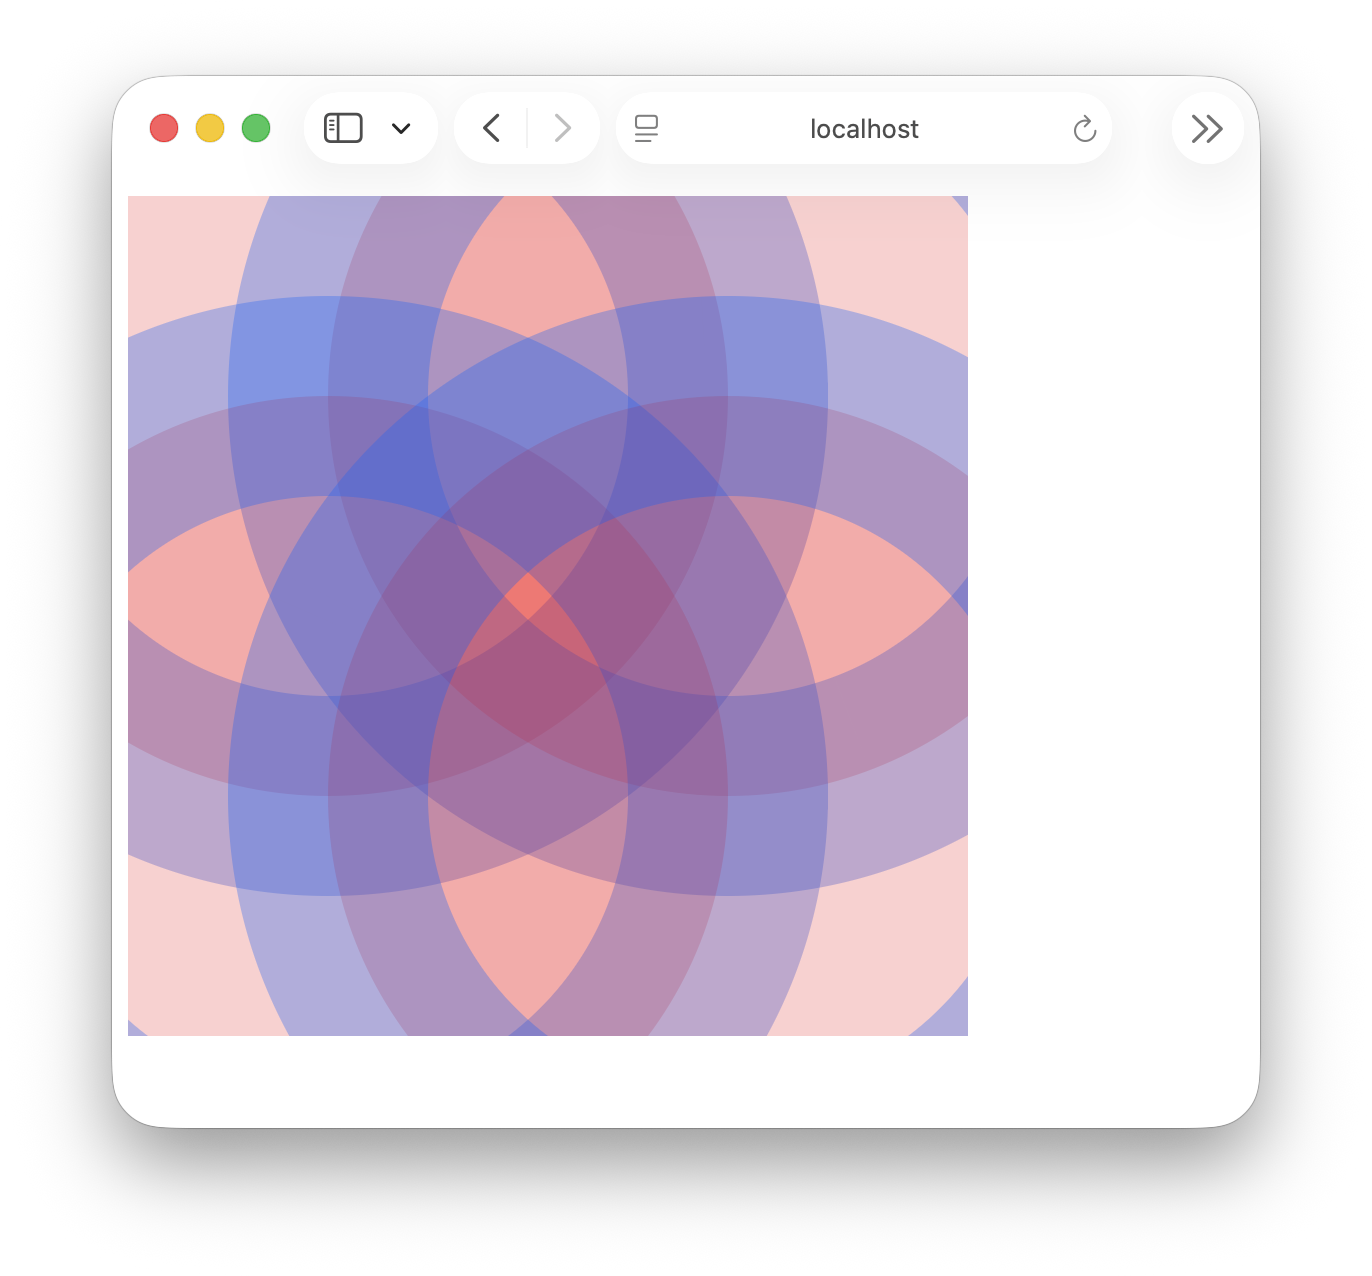
\includegraphics[width=0.5\linewidth]{figures/chapter03/transparent-color-wrapped.png}
    \caption{透明度を指定して色を重ねる（別の例）}
    \label{fig:chapter03-transparent-color-wrapped}
\end{figure}

\begin{notebox}{透明度は少しずつ試す}
透明度の値は、最初は\texttt{80}、\texttt{150}、\texttt{220}のように大きく変えて試すと違いが分かりやすくなります。
\end{notebox}

\section{色を使って顔を描く}

第2章では、円、三角形、線を組み合わせて顔のような絵を描きました。
ここでは、その絵に色と線の太さを加えて、より見た目を分かりやすくします。

\begin{listing}[htbp]
\inputminted{ts}{listings/chapter03/colored-face.ts}
\caption{色と線を使って顔を描く}
\label{lst:chapter03-colored-face}
\end{listing}

このサンプルでは、顔、目、鼻、口を描く前に、それぞれの部品に合った色を指定しています。
最後の口では、線の色と太さを指定してから\texttt{line}関数で描いています。

\begin{pointbox}{色指定の考え方}
RGBを指定するときは赤、緑、青の3つの数値を書きます。灰色は1つの数値で指定でき、4つ目の数値を加えると透明度を指定できます。
\end{pointbox}

\section{よくある間違い}

色や線の指定では、文法の間違いだけでなく、設定が残ることを忘れて起こる間違いが多くあります。思った色にならないときは、描画命令の直前を読み直しましょう。

\begin{mistakebox}{RGBの順番を取り違える}
\texttt{p.fill(255, 0, 0)}は赤、\texttt{p.fill(0, 255, 0)}は緑、\texttt{p.fill(0, 0, 255)}は青です。数値の順番は赤、緑、青です。
\end{mistakebox}

\begin{mistakebox}{色を図形の後に指定する}
\texttt{p.circle(...)}の後に\texttt{p.fill(...)}を書いても、その円の色は変わりません。色の指定は、図形を描く前に書きます。
\end{mistakebox}

\begin{mistakebox}{noStrokeの後に枠線を戻し忘れる}
\texttt{p.noStroke()}を使った後、再び枠線を描きたい場合は\texttt{p.stroke(...)}を指定します。設定は次の図形にも残ります。
\end{mistakebox}

\begin{mistakebox}{透明度の値を小さくしすぎる}
アルファ値が小さすぎると、図形がほとんど見えなくなります。まずは\texttt{150}前後から試すと分かりやすいです。
\end{mistakebox}

\section{まとめ}

この章では、RGBによる色指定、灰色系の簡易指定、塗りつぶし、枠線、線の太さ、透明度を学びました。
図形の色などの見た目は、\texttt{fill}関数、\texttt{stroke}関数、
\texttt{strokeWeight}関数などを使って変更できます。

また、色や線の設定は、次に変更するまで残ることも確認しました。複数の図形を描くときは、図形を描く直前に必要な設定が書かれているか確認する習慣をつけましょう。

\section{演習問題}

この章の演習では、色と線の指定を少しずつ変えながら、見た目の違いを確認します。最後は、自分で配色を考えた作品を作ってみましょう。

\begin{enumerate}
    \item \texttt{p.background(255)}の数値を変えて、背景を黒、灰色、白にしてください。
    \item \texttt{p.fill(255, 0, 0)}、\texttt{p.fill(0, 255, 0)}、\texttt{p.fill(0, 0, 255)}を使い、赤、緑、青の図形を描いてください。
    \item \texttt{p.fill(200)}のような1つの数値を使い、明るさの違う灰色の長方形を3つ描いてください。
    \item \texttt{strokeWeight}関数の引数の数値を変えて、細い線と太い線を描いてください。
    \item \texttt{noFill}関数を使い、塗りつぶしのない円と長方形を描いてください。
    \item \texttt{noStroke}関数を使い、枠線のない図形を3つ描いてください。
    \item \texttt{fill}関数を書く位置を変えて、どの図形の色が変わるか確認してください。
    \item 透明度を使って、2つ以上の図形が重なって見える絵を作ってください。
    \item 第2章で作った顔のサンプル\ref{lst:chapter02-simple-face}に、背景色、顔の色、目の色、口の色を追加してください。
    \item 挑戦問題として、同じ図形の組み合わせを使い、配色だけで「明るい雰囲気」と「暗い雰囲気」の2種類の作品を作ってください。
\end{enumerate}
